% This file was created by tikzplotlib v0.9.1.
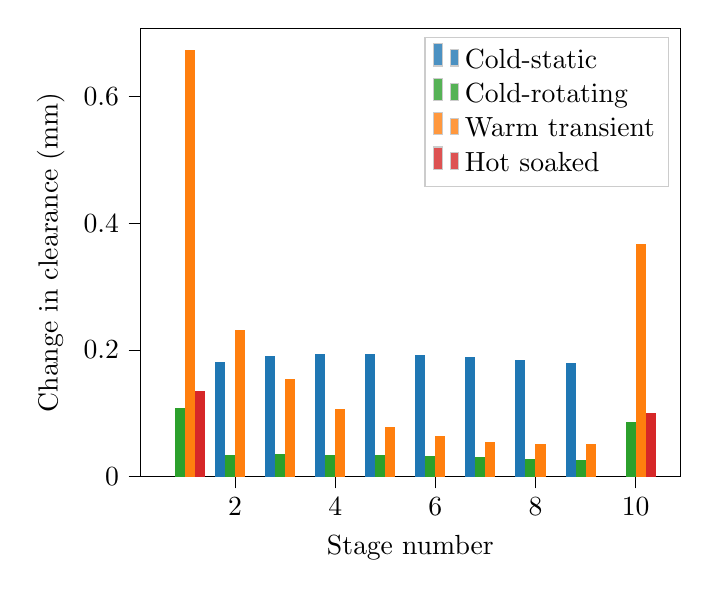
\begin{tikzpicture}

\definecolor{color0}{rgb}{0.12156862745098,0.466666666666667,0.705882352941177}
\definecolor{color1}{rgb}{0.172549019607843,0.627450980392157,0.172549019607843}
\definecolor{color2}{rgb}{1,0.498039215686275,0.0549019607843137}
\definecolor{color3}{rgb}{0.83921568627451,0.152941176470588,0.156862745098039}

\begin{axis}[
legend cell align={left},
legend style={fill opacity=0.8, draw opacity=1, text opacity=1, draw=white!80!black},
tick align=outside,
tick pos=left,
x grid style={white!69.0196078431373!black},
xlabel={Stage number},
xmin=0.11, xmax=10.89,
xtick style={color=black},
y grid style={white!69.0196078431373!black},
ylabel={Change in clearance (mm)},
ymin=0, ymax=0.708282669935342,
ytick style={color=black}
]
\draw[draw=none,fill=color0] (axis cs:0.6,0) rectangle (axis cs:0.8,0);
\addlegendimage{ybar,ybar legend,draw=none,fill=color0};
\addlegendentry{Cold-static}

\draw[draw=none,fill=color0] (axis cs:1.6,0) rectangle (axis cs:1.8,0.181108065137733);
\draw[draw=none,fill=color0] (axis cs:2.6,0) rectangle (axis cs:2.8,0.190747183051097);
\draw[draw=none,fill=color0] (axis cs:3.6,0) rectangle (axis cs:3.8,0.193999980275016);
\draw[draw=none,fill=color0] (axis cs:4.6,0) rectangle (axis cs:4.8,0.193950689816736);
\draw[draw=none,fill=color0] (axis cs:5.6,0) rectangle (axis cs:5.8,0.19190591256001);
\draw[draw=none,fill=color0] (axis cs:6.6,0) rectangle (axis cs:6.8,0.18849161447344);
\draw[draw=none,fill=color0] (axis cs:7.6,0) rectangle (axis cs:7.8,0.184111717849475);
\draw[draw=none,fill=color0] (axis cs:8.6,0) rectangle (axis cs:8.8,0.178970734041251);
\draw[draw=none,fill=color0] (axis cs:9.6,0) rectangle (axis cs:9.8,0);
\draw[draw=none,fill=color1] (axis cs:0.8,0) rectangle (axis cs:1,0.108666454716612);
\addlegendimage{ybar,ybar legend,draw=none,fill=color1};
\addlegendentry{Cold-rotating}

\draw[draw=none,fill=color1] (axis cs:1.8,0) rectangle (axis cs:2,0.0344363024147778);
\draw[draw=none,fill=color1] (axis cs:2.8,0) rectangle (axis cs:3,0.0351494260814064);
\draw[draw=none,fill=color1] (axis cs:3.8,0) rectangle (axis cs:4,0.0345967963542168);
\draw[draw=none,fill=color1] (axis cs:4.8,0) rectangle (axis cs:5,0.0334230159368468);
\draw[draw=none,fill=color1] (axis cs:5.8,0) rectangle (axis cs:6,0.0319048237698344);
\draw[draw=none,fill=color1] (axis cs:6.8,0) rectangle (axis cs:7,0.0301792294013977);
\draw[draw=none,fill=color1] (axis cs:7.8,0) rectangle (axis cs:8,0.0283343354680632);
\draw[draw=none,fill=color1] (axis cs:8.8,0) rectangle (axis cs:9,0.0264192230779111);
\draw[draw=none,fill=color1] (axis cs:9.8,0) rectangle (axis cs:10,0.08624245527131);
\draw[draw=none,fill=color2] (axis cs:1,0) rectangle (axis cs:1.2,0.674554923747945);
\addlegendimage{ybar,ybar legend,draw=none,fill=color2};
\addlegendentry{Warm transient}

\draw[draw=none,fill=color2] (axis cs:2,0) rectangle (axis cs:2.2,0.231163057322073);
\draw[draw=none,fill=color2] (axis cs:3,0) rectangle (axis cs:3.2,0.153759496450184);
\draw[draw=none,fill=color2] (axis cs:4,0) rectangle (axis cs:4.2,0.106466045132863);
\draw[draw=none,fill=color2] (axis cs:5,0) rectangle (axis cs:5.2,0.0788138225927229);
\draw[draw=none,fill=color2] (axis cs:6,0) rectangle (axis cs:6.2,0.0635483703964872);
\draw[draw=none,fill=color2] (axis cs:7,0) rectangle (axis cs:7.2,0.0553636695571235);
\draw[draw=none,fill=color2] (axis cs:8,0) rectangle (axis cs:8.2,0.0520502784991526);
\draw[draw=none,fill=color2] (axis cs:9,0) rectangle (axis cs:9.2,0.05094901611897);
\draw[draw=none,fill=color2] (axis cs:10,0) rectangle (axis cs:10.2,0.367802486114575);
\draw[draw=none,fill=color3] (axis cs:1.2,0) rectangle (axis cs:1.4,0.135147857071514);
\addlegendimage{ybar,ybar legend,draw=none,fill=color3};
\addlegendentry{Hot soaked}

\draw[draw=none,fill=color3] (axis cs:2.2,0) rectangle (axis cs:2.4,0);
\draw[draw=none,fill=color3] (axis cs:3.2,0) rectangle (axis cs:3.4,0);
\draw[draw=none,fill=color3] (axis cs:4.2,0) rectangle (axis cs:4.4,0);
\draw[draw=none,fill=color3] (axis cs:5.2,0) rectangle (axis cs:5.4,0);
\draw[draw=none,fill=color3] (axis cs:6.2,0) rectangle (axis cs:6.4,0);
\draw[draw=none,fill=color3] (axis cs:7.2,0) rectangle (axis cs:7.4,0);
\draw[draw=none,fill=color3] (axis cs:8.2,0) rectangle (axis cs:8.4,0);
\draw[draw=none,fill=color3] (axis cs:9.2,0) rectangle (axis cs:9.4,0);
\draw[draw=none,fill=color3] (axis cs:10.2,0) rectangle (axis cs:10.4,0.100430149917291);
\end{axis}

\end{tikzpicture}
